% Created 2020-05-06 mié 13:47
% Intended LaTeX compiler: pdflatex
\documentclass[a4paper, 12pt]{article}
\usepackage[utf8]{inputenc}
\usepackage[T1]{fontenc}
\usepackage{graphicx}
\usepackage{grffile}
\usepackage{longtable}
\usepackage{wrapfig}
\usepackage{rotating}
\usepackage[normalem]{ulem}
\usepackage{amsmath}
\usepackage{textcomp}
\usepackage{amssymb}
\usepackage{capt-of}
\usepackage{hyperref}
\usepackage{float, amsfonts, commath, mathtools}
\author{Tabaré Pérez}
\date{\today}
\title{Lecture 13 - 6: Similarity Measures-Cost functions}
\hypersetup{
 pdfauthor={Tabaré Pérez},
 pdftitle={Lecture 13 - 6: Similarity Measures-Cost functions},
 pdfkeywords={},
 pdfsubject={},
 pdfcreator={Emacs 26.3 (Org mode 9.3.6)}, 
 pdflang={English}}
\begin{document}

\maketitle
So the question that we now need to discuss is how to define the clustering
cost.

And this is a real question. Let's consider the following sequence of points.
I'm intentionally going to draw twice the same points.

This is one set of your points, and I am copying it as much as I could to make it
look similar:

\begin{figure}[H]
\centering
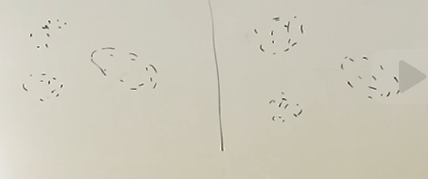
\includegraphics[width=0.5\textwidth]{./pic/04-06-fig-01.png}
\caption{\label{fig:org3930fde}Fig. 01}
\end{figure}

So looking at these points, let's say I'm forced to divide it into two clusters.
Somebody told me I have to divided into two clusters. So maybe I can divide them
this way into two clusters.

\begin{figure}[H]
\centering
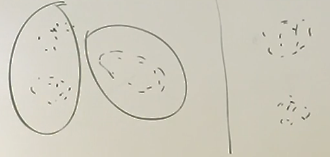
\includegraphics[width=0.5\textwidth]{./pic/04-06-fig-02.png}
\caption{\label{fig:orgf38c0b3}Fig. 02}
\end{figure}

Alternatively, I can divide them this way into two clusters.

\begin{figure}[H]
\centering
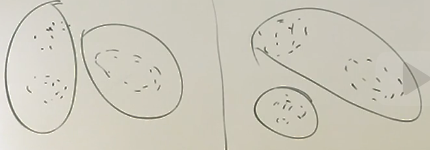
\includegraphics[width=0.5\textwidth]{./pic/04-06-fig-03.png}
\caption{\label{fig:org205916d}Fig. 03}
\end{figure}

So how do I know which one of them is better? So I need to have a cost which
will take any possible partitioning of this points and tell me, this one has
cost 5, this one maybe has cost 2, that's why this one is preferable for me.

\begin{figure}[H]
\centering
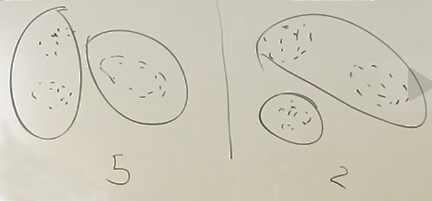
\includegraphics[width=0.5\textwidth]{./pic/04-06-fig-04.png}
\caption{\label{fig:orge084be1}Fig. 04}
\end{figure}

So what we will need to do, and let's just look one step farther where we are
going with it in the lecture, if we have this kind of cost, we can then look at
the optimization algorithm which will go and find the best partitioning with
this cost. But first of all, we need to decide how do we define the cost?

And there are many, many ways to define the cost of the partitioning.

So the general assumption that we will make here, when we are looking at the
cost of a specific partitioning, (and you notice I'm going for \(1\) to \(K\)
because we have \(K\) clusters) we would assume that it will be sum of the costs
of individual clusters:

\begin{equation}
\text{cost}(C_1 \ldots C_K) = \sum_{j=1}^{K}\text{cost}(C_j)
\end{equation}

So in other words, it's very intuitive that you would say, the goodness of this
whole partition would be sum of how good is every individual cluster.

So now we reduce our question to the question of cost of the specific clusters.
For instance, here we are looking at the specific cluster and we need to define
its cost.

\begin{equation}
\text{cost}(C)
\end{equation}

This is a specific cluster. So how can we define cost? Again, there are many
ways. In some ways, this cost should reflect how homogeneous, how consistent is
this cluster. For instance, if we look at a specific cluster, we can ask how far
are the most remote points. We can look at the \textbf{DIAMETER}:

\begin{equation}
\text{cost}(C) = \text{DIAMETER}
\end{equation}

This is option one. We can do something else. We can look the average distance
between all the points:

\begin{equation}
\text{cost}(C) = \left\{ \begin{array}{l}
                          \text{DIAMETER} \\
                          \text{AVERAGE DISTANCE}
                         \end{array} \right.
\end{equation}

And you already can see that whenever you are committing to specific
measurements usually defining how it would look like:
\begin{itemize}
\item If you're looking at the diameter, then the outlier will be determining your
cost.
\item If you look at average distance and all the members in some way will be
contributing.
\end{itemize}

The measures, the cost that I would like to introduce today, which we would use
very commonly would actually bring in these representatives, and what this
measure will do, it will determine the cost of the cluster by comparing the
distance between all the members of the cluster and the specific representative.
It means that whenever I am giving you a specific cluster, I have to give you
the representative because then you would be able to go and compute for me the
cost. So given some class \(C\) and a particular representative \(z\), I would
just say that my cost would be:

\begin{equation}
\text{cost}(C,z) = \sum_{i \in C} \text{distance}(x^{(i)}, z)
\end{equation}

 The sum for all the points \(i\) in \(C\) of some measurements of distance
between \(x^{(i)}\) and \(z\).

So we went through all the points that belong to this particular cluster and
compare its distance with the representative \(z\).

So now the question of computing the cost of a cluster reduced to a question of
computing the similarity of the distance between two vectors, like in this case,
between the representative and a specific point in a cluster.

So the first similarity measures that I will introduce you may have seen in many
other contexts. It's called \textbf{COSINE SIMILARITY}.

What it does, it takes two vectors and looks at the angle between these two
vectors. So in this case, if you're given a vector \(x^{(i)}\) and the vector
\(x^{(j)}\), then the cosine similarity between them would be their
corresponding dot product divided by the product of their norms:

\begin{equation}
cos(x^{(i)}, x^{(j)}) = \frac{x^{(i)} \cdot x^{(j)}}{\norm{x^{(i)}} \norm{x^{(j)}}}
\end{equation}

Another common measures that is used is actually a distance. Not a similarity, a
distance metric which just looks at the distance between points in the space and
it's called \textbf{EUCLIDEAN SQUARED DISTANCE}:

\begin{equation}
\text{distance}(x^{(i)}, x^{(j)})^2 = \norm{x^{(i)} - x^{(j)}}^2
\end{equation}

\begin{equation}
\text{distance}(x^{(i)}, x^{(j)})^2 = [U - V]^\intercal \cdot [U - V]
\end{equation}

So this distance measure takes again, two points, and looks at the square of
that norm.

Now let's just look at this two different ways to compare vectors in order to
understand the difference.

So, for instance, the cosine similarity is not sensitive to the magnitude of the
vectors. So what it tells us, for instance, in terms of our Google News
application, that if we choose cosine to compare between two vectors
representing two different stories, that this measurement will not take it into
account how long is the story.

On the other hand, Euclidean distance will be sensitive to the lengths of the
story.

And there are lots and lots of other measurements that you can find in the
literature.

I would be using the Euclidean square distance and you would shortly discover
why.

But the questions that you need to be asking yourselves, and I will ask you
later, is what makes the match between the similarity measure and the algorithm
and when it is important and when it is not important.

But at any rate, let's say I convinced you at this point to pick up Euclidean
squared distance.

And now I want to write for you the cost of the partitioning.

I am coming back to this question, how to compute the cost of the partitioning?
And as I said earlier, what I would want to do, I would want to define the cost
of the partitioning in terms of the distance, in this case, Euclidean squared
distance between the elements of the cluster and the representative.

So in order for me to write this cost, now it is not enough to write just the
partitions themselves. I need to have also the representatives. So you would be
given a partitioning of \(K\) clusters and then \(K\) representatives. And we will use
squared Euclidean distance to go over every single cluster. That's what I'm going
to do. I am going to go from cluster \(1\) to cluster \(K\). And then, within each
cluster, I will take the points that belong to this cluster, all the indexes of
points that belong to cluster \(C_j\), and then compute squared Euclidean distance
between this point and the representative of this cluster:

\begin{equation}
\text{cost}(C_1 \ldots C_K, z^{(1)}, \ldots ,z^{(K)}) = \sum_{j=1}^{K} \sum_{i \in C_j} \norm{x^{(i)} - z^{(j)}}^2
\end{equation}

And you may be looking at it and thinking, why do I need to carry both? Maybe I
can compute representative if I know the clusters. This is true. And as we will
continue our lecture, we will see how to unify them together. But at this point,
I would want you to think about this cost, which we will be optimizing.

I would assume that we are given the clusters, we are given the representatives,
and this is our way to compute the cost with squared Euclidean distance.
\end{document}